\chapter{Equipment \& Combat Techniques}
Weapons and armor offer a variety of combat options to those skilled in their use. Each weapon and weapon type has certain properties that affect the manner in which it is used and the effects it has on targets. Players are encouraged to explore different choices of armament to see which tactics are effective in which situations. You may find that certain weapon types are more effective against certain enemies; it is therefore advantageous to train multiple combat skills and use the right weapons for the job.\\

In addition to these basic properties, equipment also grants access to combat techniques --- special moves you can do that deal extra damage and have bonus effects. Most techniques become available as your skill with weapons increases, as described in the skill mastery perk table (\textit{section 3.2}). Some techniques are available to everyone and may be used regardless of which weapons one is wielding. However, combat techniques cost stamina, so be sure to pace yourself!

\section{Glossary of Weapon Properties}
\begin{itemize}
	\item \textbf{Blade}: This is a bladed weapon, and it uses the Blade skill for attack rolls. All bladed weapons are Impaling.
	\item \textbf{Blunt}: This is a blunt weapon, and it uses the Blunt skill for attack rolls. Blunt weapons ignore some armor points.
	\item \textbf{Heavy}: This weapon is so large and/or heavy that it cannot be used more than once per round under any conditions.
	\item \textbf{Impaling}: This weapon has a sharp edge or point; on an extreme success, weapons with this property deal max damage and then another base damage die. (e.g. a longsword (1d10+DB) deals 10 damage in addition to the normal damage bonus and another d10 roll.)
	\item \textbf{Light}: This weapon is small and light enough that it can be used up to three times in a round. It is also excellent for dual wielding.
	\item \textbf{Magic}: This weapon has magical properties which may make it interact with certain enemies in unusual ways.
	\item \textbf{Marksman}: This is a bow, and it uses the Marksman skill. All bows are Impaling.
	\item \textbf{Medium}: This weapon's weight is between that of a light and a heavy weapon, and it can be used twice per round.
	\item \textbf{One-Handed}: This weapon only requires one hand to use.
	\item \textbf{Reach}: This weapon's length extends your reach by 5 ft.
	\item \textbf{Two-Handed}: This weapon requires the use of two hands and therefore prevents dual wielding, the use of shields, and possibly other tasks requiring hands (at the GM's discretion).
\end{itemize}

In addition to these properties, specific weapons also have a Quality, which can grant extra damage compared to poorer weapons of the same type. They have a base damage die as well, listed before the properties. Remember to add your skill and attribute damage bonuses as well. You get +1 to all melee attacks for every 25 points of Strength and +1 to all ranged attacks for every 25 points of Agility. Skills work the same way: every 25 points in a skill gives you a permanent +1 damage bonus for all weapons covered by that skill.\\

\begin{tcolorbox}
	\textbf{Note}: whenever you see the abbreviation ``DB'', this refers to your damage bonus, which is the extra damage you gain via your attributes and skills. Extra damage granted by weapon quality is considered part of that weapon's base damage. Damage granted by enchantments or poisons is added after all multipliers are calculated and is not considered part of the damage bonus.
\end{tcolorbox}

\begin{figure}[h]
	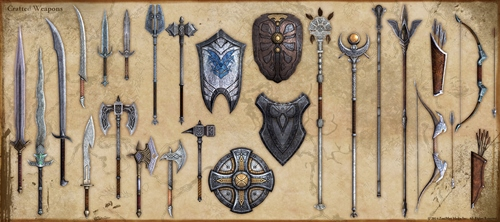
\includegraphics[width=\textwidth]{Equipment.png}
\end{figure}

\section{Combat Techniques}

Combat techniques are special maneuvers that you can perform while in combat, allowing you to do more than just move and swing a weapon. Combat techniques generally require an action to execute and cost stamina. Techniques labeled as "Reaction" can be executed in response to a specific event instead of using an action on your turn. Each reaction technique imposes an additional penalty die on the next one until your next turn. For example, if you have dodged and fought back between turns, attempting to dodge again will be an Acrobatics check with two penalty dice (in addition to any that may be imposed by other circumstances).

\subsection{Common Techniques}

While certain combat techniques will only be available to skilled warriors while wielding specific weapons, some techniques are available to everyone and can be used with various different weapons.

\begin{itemize}
	\item \textbf{Block} (\textit{10 Stamina, Reaction}): If you are targeted by a melee attack, you may attempt to block it. Make an opposed Block check. On a success, you block the attack and take no damage.
	\item \textbf{Dive for Cover} (\textit{Free, Reaction}): When you first notice an enemy, you may dive for the ground as a reaction, preferably behind cover. Otherwise, this technique costs an Action. You are able to cover 10 feet using this move, and you go prone as a result. This move imposes a penalty on ranged attack rolls targeting you.
	\item \textbf{Dodge} (\textit{10 Stamina, Reaction}): If you are targeted by a melee attack, you may attempt to dodge by making an opposing Acrobatics check. On a success, you dodge the opponent's attack entirely and take no damage. On a tie, the dodger wins.
	\item \textbf{Dual Wield Attacks} (\textit{Free, Bonus Action}): If you attack with a light, one-handed weapon and are holding another light, one-handed weapon, you may attack with the latter as a bonus action; however, the second attack does not benefit from your damage bonus. If you use Flurry of Blows while dual wielding, each weapon gets only two attacks, for a total of four. The damage bonus rule still applies to your off-hand weapon in this case.
	\item \textbf{Fight Back} (\textit{10 Stamina, Reaction}): You respond to incoming melee attacks with attacks of your own. You must be within range of the attacker and not otherwise unable to attack. You can only make one attack, it may not be a combat technique. On a success, you avoid coming to harm and your attacker suffers damage. On a tie or failure, your attack fails to land and your attacker successfully strikes you.
	\item \textbf{Flurry of Blows} (\textit{60 Stamina, Action}): You swing your weapon(s) quickly, dealing multiple blows in a single round. Light weapons may attack 3 times, medium weapons may attack twice, and heavy weapons may not use this technique. For the purpose of successive reaction penalty dice, this technique counts as one attack.
	\item \textbf{Grapple} (\textit{20 Stamina, Action}): If you have at least one free hand, you may attempt to grab your target. Make a melee attack using your Athletics skill. You do no damage, but the target is grappled on a success. A grappled target cannot move. Your speed while holding an unwilling creature is halved. A grappled creature may attempt to break free with its action using an opposed Athletics check.
	\item \textbf{Opportunity Attack} (\textit{10 Stamina, Reaction}): If a combatant leaves your melee range during their turn, you may react by making a single attack against them.
	\item \textbf{Sneak Attack} (\textit{Free, Action}): If you are undetected, you may attack a target for bonus damage determined by your Sneak skill (\textit{see section 3.2}). Sneak attacks always gain a bonus die, but their damage multipliers do not stack with those of other combat techniques.
\end{itemize}

\subsection{Weapons \& Skill-Based Combat Techniques}

The following sections describe different types of weapons and the combat techniques associated with that weapon type. Please note that the weapon types listed are merely types and not specific weapons; while all weapons of that type you find in the game will have the listed properties, some features might vary. Also, for every melee technique listed in this section, the following applies: if your target successfully rolls to block your attack and you used a light weapon to make it, the target is recoiled.

\subsubsection{Blade}

Bladed weapons are deadly in the hands of highly skilled wielders thanks to their \textit{Impaling} property. They tend to be more effective against poorly armored opponents thanks to the ease with which blades can cut through flesh compared to the effects of blunt weapons. Bladed weapons in the Elder Scrolls Tabletop RPG come in four varieties:

\begin{itemize}
	\item \textbf{Daggers} (\textit{1d6, Light, One-Handed}): Blades shorter than the forearm. Not very effective against armor, but incredibly deadly in the hands of an adept sneak.
	\item \textbf{Shortswords} (\textit{1d8, Light, One-Handed}): Short, thin bladed swords. More effective than daggers in open combat, but less optimal for sneak attacks.
	\item \textbf{Longswords} (\textit{1d10, Medium, One-Handed}): Long, somewhat heavy blades designed for one- or two-hand grips. Not as quick as a shortsword or dagger, but weighty enough to fare well against armor.
	\item \textbf{Claymores} (\textit{2d6, Heavy, Two-Handed, Reach}): Very long and heavy blades that must be wielded with two hands in order to use them effectively. Great for heavy combat and punching holes in armor at the cost of slow swings.
\end{itemize}

Blade techniques are primarily focused on dealing as much damage as possible. They become available every 25 skill points in Blade as specified in the mastery perk table (\textit{section 3.2}). Each of these techniques costs 60 stamina to execute. If a target successfully blocks a blade technique you made with a medium or heavy blade, they receive recoil. Thus, even failing to land these big hits can come with some benefits. The five blade techniques are:

\begin{itemize}
	\item \textbf{Power Attack}: You wind up and unleash a heavy blow, doubling your damage.
	\item \textbf{Standing Strike}: You plant your feet and strike with all your might, tripling your damage at the cost of being unable to move on the same turn.
	\item \textbf{Flanking Strike}: You swing your weapon broadly across the area in front of you, doubling your damage and allowing you to attack two adjacent targets within reach. (You only roll attack once; each target rolls block/dodge against that number, and attacks are resolved individually.)
	\item \textbf{Sweeping Attack}: You aim low, attempting to strike at your opponent's legs. Damage is doubled; on an extreme success, your opponent is knocked prone.
	\item \textbf{Dizzying Blow}: You swing directly for your opponent's head. Damage is doubled. On an extreme success, your opponent is paralyzed until the end of their next turn.
\end{itemize}

\subsubsection{Blunt}

In general, blunt weapons are more effective against armor due to the manner in which they bludgeon weak points. However, they do not get the \textit{Impaling} bonus to extreme successes; instead, they merely deal max damage. There are four types of blunt weapons:

\begin{itemize}
	\item \textbf{War Axes} (\textit{1d8, Light, One-Handed}): Hand-sized axes, light and quick for blunt weapons. Their weight makes them better at penetrating armor than other light weapons.
	\item \textbf{Maces} (\textit{1d10, Medium, One-Handed}): Bludgeons with a weighty head at the end of a handle. Useful for crumpling skulls and armor alike. Not quite as swift as war axes, but significantly more effective against armored foes.
	\item \textbf{Battleaxes} (\textit{1d12, Heavy, Two-Handed, Reach}): Big, heavy axes that require both hands to swing. Great for cleaving limbs and leaving deep,  grievous wounds.
	\item \textbf{Warhammers} (\textit{2d6, Heavy, Two-Handed, Reach}): Huge hammers intended not for construction but smashing foes. Allows for consistently forceful strikes.
\end{itemize}

Blunt techniques are identical to Blade techniques, except they become available via advancement in the Blunt skill. Again, each technique costs 60 stamina to execute, and if a target successfully blocks one of these attacks made with a medium or heavy weapon, they receive recoil. The five blunt techniques are:

\begin{itemize}
	\item \textbf{Power Attack}: You wind up and unleash a heavy blow, doubling your damage.
	\item \textbf{Standing Strike}: You plant your feet and strike with all your might, tripling your damage at the cost of being unable to move on the same turn.
	\item \textbf{Flanking Strike}: You swing your weapon broadly across the area in front of you, doubling your damage and allowing you to attack two adjacent targets within reach. (You only roll attack once; each target rolls block/dodge against that number, and attacks are resolved individually.)
	\item \textbf{Sweeping Attack}: You aim low, attempting to strike at your opponent's legs. Damage is doubled; on an extreme success, your opponent is knocked prone.
	\item \textbf{Dizzying Blow}: You swing directly for your opponent's head. Damage is doubled. On an extreme success, your opponent is paralyzed until the end of their next turn.
\end{itemize}

\subsubsection{Hand-to-Hand Techniques}

Unarmed attacks deal less damage than blade, blunt and marksman weapons. They do not benefit from the Impaling property, nor do they get to ignore armor points like blunt weapons. They also deal less base damage than any of the listed weapons (\textit{1d4}) and do not have benefit from weapon quality damage bonuses. However, hand-to-hand attacks have the unique benefit of exhausting the target. Whenever you deal damage with an unarmed attack, half of that damage is also removed from the target's stamina. Unarmed attacks also count as light weapons and so benefit from Flurry and dual wielding. Hand-to-Hand techniques are similar to melee weapon techniques, but they are more focused on disrupting the enemy. Like the previous categories, each technique listed here costs 60 stamina to execute.

\begin{itemize}
	\item \textbf{Power Attack}: You wind up and unleash a heavy blow, doubling your damage.
	\item \textbf{Standing Strike}: You plant your feet and strike with all your might, tripling your damage at the cost of being unable to move on the same turn.
	\item \textbf{Disarming Attack}: You strike viciously at your opponent's weapon arm. Your attack deals double damage, and the opponent is disarmed on an extreme success.
	\item \textbf{Paralyzing Palm}: You strike at your opponent's vitals, causing them to reel in pain. Your attack deals double damage, and on an extreme success, the opponent is paralyzed until the end of their next turn.
	\item \textbf{Power Within}: You channel your inner power and strike a powerful blow against your foe. Your damage is doubled. On an extreme success, you may convert half of your damage to fire, frost or shock damage, your choice.
\end{itemize}

\subsubsection{Archery}

Bows are silent and lethal ranged weapons. Bows are often favored by stealthy characters as a way to attack enemies at range with minimal risk of exposure. Their ability to deliver poisons via arrowhead makes them especially potent; even if the arrow does not finish the job, the poison may. While blades can be poisoned and are still highly useful for this purpose, quite a bit of mischief can be caused when one is not within arm's reach. Poisons aside, bows are very precise puncturing weapons. While they are not as effective against armor as blunt weapons, they are highly deadly in the hands of trained archers. All bows in the ESTRPG have the \textit{Impaling} and \textit{Two-Handed} properties, since their arrows are sharp and pointed and bows take both hands to use. Just make sure you bring enough arrows with you! There are two types of bows in the game:

\begin{itemize}
	\item \textbf{Shortbows} (\textit{2d6, 80 ft, Medium}): Bows of modest length, generally allowing for faster draw speed at the cost of less power.
	\item \textbf{Longbows} (\textit{2d8, 150 ft, Heavy}): Bows typically as tall as the archer, with enough power to send arrows flying faster and farther at the cost of slower draw speeds.
\end{itemize}

Marksman attacks in combat use different mechanics from melee attacks; targets cannot react by dodging or blocking. Instead, a difficulty is chosen for the attack roll based on how far away the target is in relation to the weapon's base range (normal for within, hard for within double, extreme for within triple). Bonus and penalty dice are then assigned based on conditions affecting the shot. The conditions are as follows:

\begin{center}
\begin{tabular}{p{0.5\textwidth}p{0.5\textwidth}}
	Bonus
	\begin{itemize}
		\item Aiming
		\item Large target
	\end{itemize}
	&
	Penalty
	\begin{itemize}
		\item Small target
		\item Target is within melee range
		\item Target in partial cover
		\item Target diving for cover
		\item Firing into a melee with friendlies
		\item Fast-moving target (moved 50 feet or more on last turn)
	\end{itemize}\\
\end{tabular}
\end{center}

These apply to ranged attacks with any weapon or spell.\\

Marksman techniques are less concerned with dealing extra damage and more with improving archery conditions. Nonetheless, they typically do improve upon the already formidable base damage of bows.

\begin{itemize}
	\item \textbf{Aim} (\textit{10 Stamina}): By staying still for a round and taking no damage, you are able to concentrate and line up a good shot. Your next attack has a bonus die and +20 ft to base range.
	\item \textbf{Volley} (\textit{60 Stamina}): You can fire two arrows in one round when using a shortbow.
	\item \textbf{Trick Shot} (\textit{60 Stamina}): Your attack deals double damage and ignores penalty dice imposed by partial cover.
	\item \textbf{Focus Shot} (\textit{60 Stamina}): Your attack deals double damage and ignores penalty dice imposed by firing into a melee.
	\item \textbf{Snipe} (\textit{60 Stamina}): Your attack deals triple damage, and base range is increased by 25\% for this attack. Range bonus does not stack with Aim.
\end{itemize}

\begin{tcolorbox}
\textbf{Note}: You have a limited number of arrows, so be careful with your attacks. It is assumed you are able to recover all your arrows after combat unless something happens to them.
\end{tcolorbox}

\begin{figure}[h]
	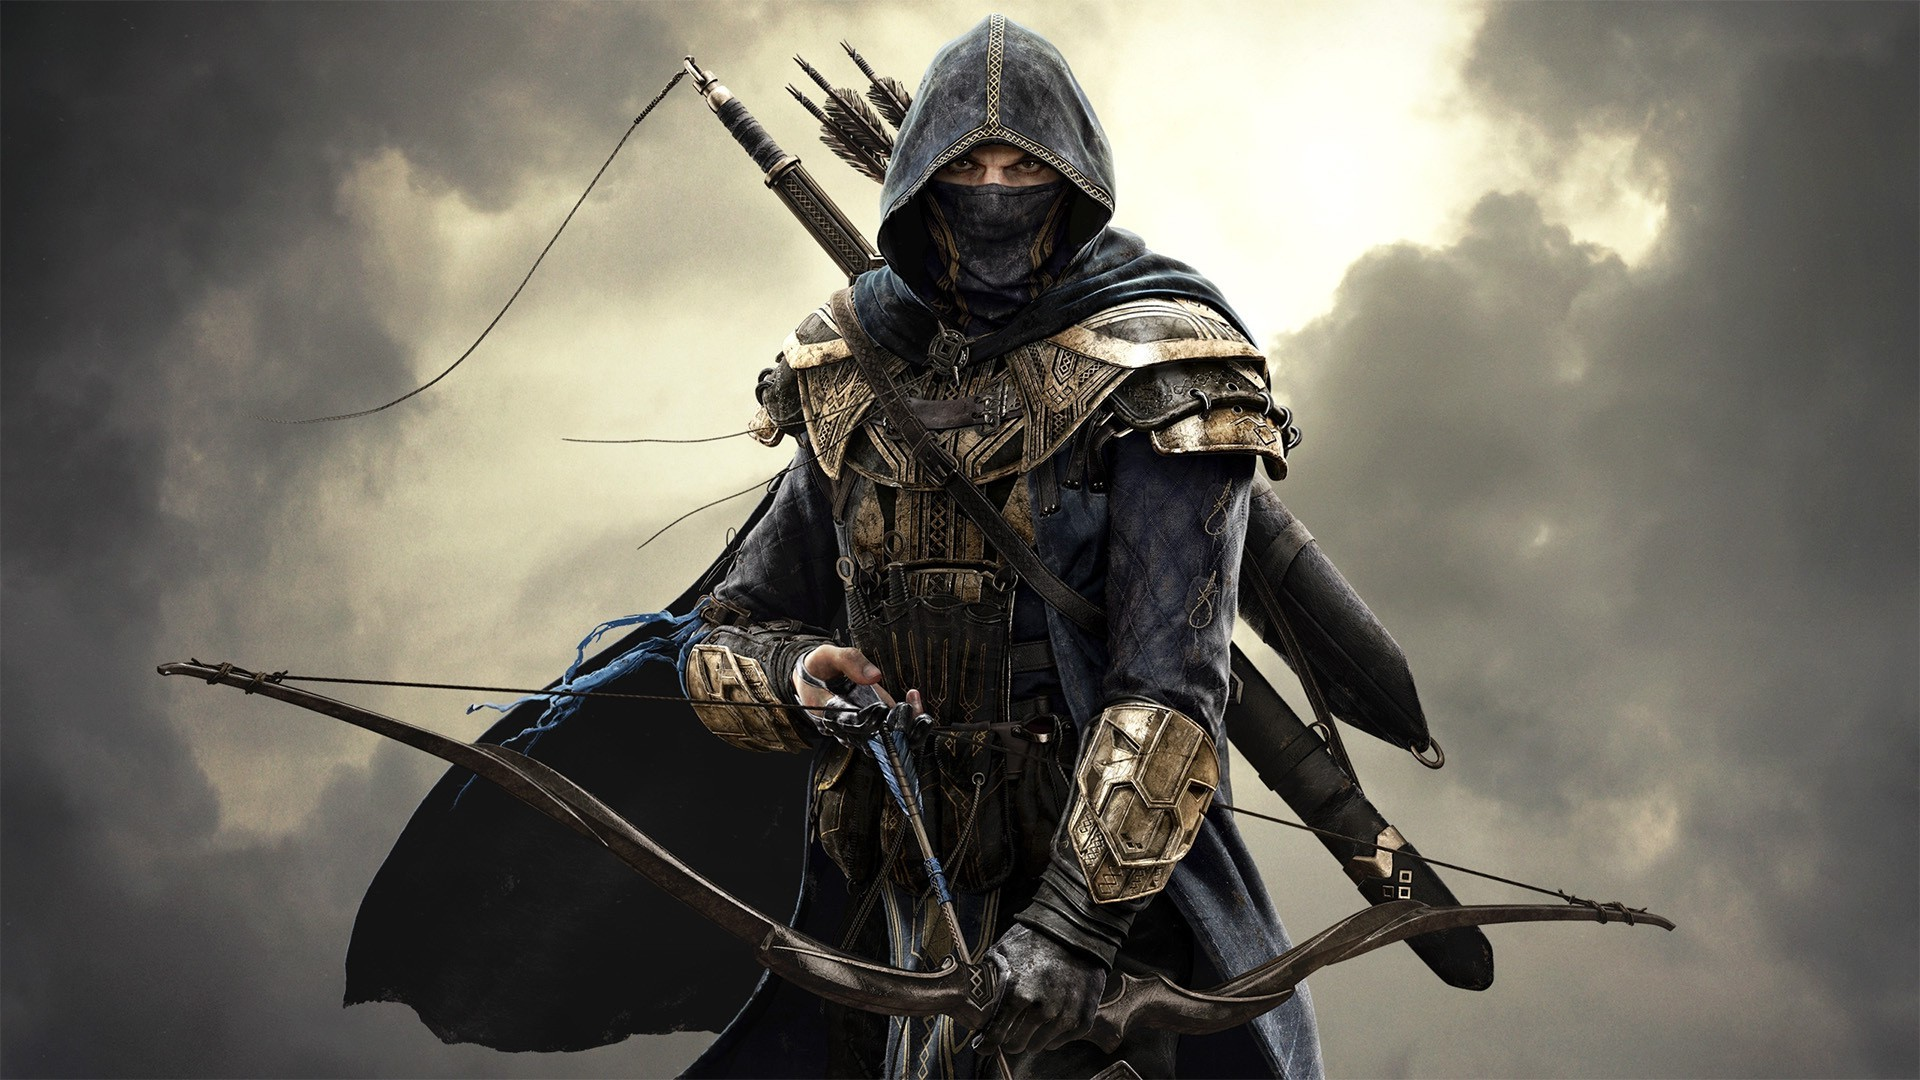
\includegraphics[width=\textwidth]{bretonarcher.png}
\end{figure}

\section{Armors \& Shields}

Armor is quite simple in the ESTRPG. Rather than splitting armor up into various pieces and requiring the player to find them all, armors come in full suits. Each armor has an armor rating. whenever you take physical damage while wearing armor, subtract that armor's rating from the damage. Armor rating does not decrease from attacks unless something special damages the armor.\\

Armor comes in two varieties: heavy and light. Heavy armor generally provides better protection, but it imposes a penalty die on all non-social Stealth checks. All armor reduces movement speed, but heavy armor tends to reduce it more. Armor penalties can be mitigated by improving your armor skills. Shields are sold separately, but they provide additional armor and a bonus die on block rolls.

\section{Scrolls \& Staves}

Staves have stored spells in them which you can cast without spending magicka. Using one to attack works exactly the same way as using the spell stored in it (see \textit{Chapter 6}), only you do not need to know the spell or be of sufficient level to use it. When a staff runs out of charge, you cannot cast spells with it. It can be recharged by consuming a soul gem or by bringing it to a spell merchant and paying a fee.\\

Scrolls also allow you to cast stored magic without needing to know the spell, have the skill required to use it or spend any magicka. However, scrolls only allow you to cast a single spell before they are consumed and become completely useless.

\begin{figure}[h]
	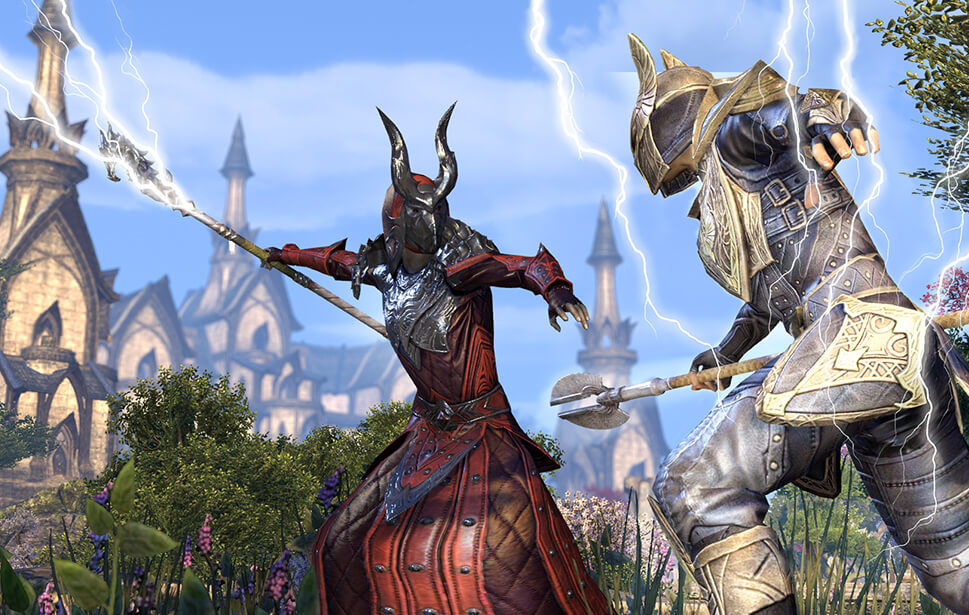
\includegraphics[width=\textwidth]{staves.png}
\end{figure}

\section{Improvised Weapons}
Sometimes, you may find yourself in a fight with no weapons on hand. Some objects may be used as improvised weapons and should be treated as a similar weapon type for the purposes of attacking. A chair leg might be defined as a mace, for example. The GM will decide what stats the item receives in this case. An object that does not resemble a weapon deals 1d6 damage.

\section{Silver Weapons}
You may come across certain creatures who are immune to normal weaponry. Such creatures may have be vulnerable to silver. You can pay a fee of 100 Septims to have a weapon silvered, giving it the Magic property.

\section{Adventuring Gear}
This section lists miscellaneous gear that will be useful in your adventures. Costs listed are \textit{base cost}, which will be modified according to your Mercantile skill.

\begin{itemize}
	\item Acid Vial (25 Septims, 1 lb): A small amount of acid stored in a glass vial. It can be splashed on a target within 5 feet for 2d6 physical damage that ignores armor. Items splashed by acid are damaged.
	\item Alchemical Fire (50 Septims, 1 lb): A flask of sticky fluid that ignites when exposed to air. As an action, you can throw the flask up to 20 feet. Make a Marksman check to hit a creature with the flask. On a hit, the target is ignited and takes 1d4 fire damage at the beginning of each of its turns for the next 3 rounds.
	\item Alchemist's Kit (50 Septims, 2 lbs): contains vials and space to store your potions and alchemy apparatuses.
	\item Alembic (Varying Cost, 7 lbs): Used to distill alchemical mixtures. One of four types of alchemy apparatuses; price varies with quality.
	\item Arrows --- Bundle of 20 (20 Septims, 1 lb): A set of 20 arrows. May be used with shortbows or longbows.
	\item Antitoxin (50 Septims, 1 lb): A potion in a glass bottle. Drink it to cure yourself of poison.
	\item Backpack (20 Septims, 5 lbs): While worn, a backpack allows you to carry an additional 30 lbs of equipment without overencumbering yourself.
	\item Ball Bearings --- Sack of 1,000 (10 Septims, 2 lbs): A sack filled with 1,000 tiny steel balls. You may scatter them in a 5 ft radius; any creature moving through this area that moves more than half its speed must succeed on an Acrobatics check or fall prone.
	\item Bedroll (20 Septims, 7 lbs): Provides sufficient comfort to sleep on hard ground.
	\item Blanket (5 Septims, 3 lbs): Protects you from cold while you sleep.
	\item Block and Tackle (10 Septims, 5 lbs): A set of pulleys, hooks and cables that allows you to hoist objects up to four times the weight you can normally lift.
	\item Book (Varying Cost, 5 lbs): A book containing information that could include lore, illustrations, diagrams or really anything else that can be written down on paper.
	\item Calcinator (Varying Cost, 5 lbs): A metal bowl on a stand, used in alchemical processes. One of four alchemical apparatuses. Cost varies with quality.
	\item Caltrops --- Sack of 20 (10 Septims, 2 lbs): A sack filled with small metal spike traps that always point upward no matter how they are oriented. You may scatter them in a 5 ft diameter; creatures moving more than half their speed must succeed on a hard acrobatics check or cease moving and take 5 physical damage.
	\item Candle (1 Septim, 0 lbs): For one hour, a candle will shed 5 feet of bright light and 5 feet of dim light beyond that.
	\item Case, parchment (10 Septims, 1 lb): A protective case that can hold maps, papers and parchments. No more than 10 sheets.
	\item Chain --- 10 ft (15 Septims, 10 lbs): A chain has 20 hit points. It can be broken by success on an extreme Athletics check.
	\item Climber's Kit (40 Septims, 12 lbs): A kit containing ropes, pitons, boot tips and a harness. Allows you to set up to 2 harness points from which you cannot be moved more than 25 feet, even by falling.
	\item Clothes, Common (5 Septims, 3 lbs): Clothes that would be worn by commoners. Cheap, but do not make much of an impression on the wealthy.
	\item Clothes, Costume (25 Septims, 3 lbs): Clothes specially intended to disguise you. May not hold up to close inspection.
	\item Clothes, Fine (30 Septims, 4 lbs): Clothes worn by people of means.
	\item Clothes, Traveling (10 Septims, 2 lbs): Light, durable clothing favored by people on the move.
	\item Crowbar (15 Septims, 5 lbs): Crowbars give you a bonus die on Athletics checks where strength is required and leverage may be applied.
	\item Fishing Tackle (10 Septims, 4 lbs): A set of fishing equipment, contains all you need to fish in rivers or lakes.
	\item Healer's Kit (30 Septims, 3 lbs): A leather pouch containing bandages, splints and salves. You may use this item to stabilize a dying creature. The kit has 10 uses.
	\item Hourglass (40 Septims, 1 lb): A glass container with sand inside. Turning it over allows sand to flow from one partition of the container to the other at a rate such that when it is complete, an hour will have passed.
	\item Hunting Trap (20 Septims, 25 lbs): A sawtoothed steel ring that snaps shut when activated by a pressure plate in the middle. Creatures that step on the pressure plate must succeed on an Acrobatics check to move away before the trap shuts. Otherwise, they take 1d4 physical damage and lose all movement until they are freed. A creature may attempt to break free using a hard Athletics check.
	\item Ink Bottle (40 Septims, 0 lbs): Used for writing.
	\item Ink Pen (1 Septim, 0 lbs): Also used for writing.
	\item Ladder --- 10 feet (10 Septims, 25 lbs): A pair of poles connected by rungs, allowing one to climb up them easily.
	\item Lamp (15 Septims, 1 lb): Casts bright light in a 15-ft radius and dim light an additional 30 feet. Once lit, it burns for 6 hours on a flask of oil.
	\item Lantern, Bullseye (40 Septims, 2 lbs): A lantern with a single, round opening designed to cast light in a narrow beam. The opening has an attached cover that may be shut. The lantern casts bright light in a 60-ft cone and dim light an additional 60 feet beyond that. Once it, it burns for 6 hours on a flask of oil.
	\item Lantern, Hooded (25 Septims, 2 lbs): Casts bright light in a 30-ft radius and dim light for an additional 30 ft. Once lit, it burns for 6 hours on a flask of oil. As an action, you may lower the hood to change the light level to a 5-ft radius of dim light.
	\item Lock (Varying cost, 1 lb): Locks come with keys and may be used to prevent access to doors or containers. Higher lock difficulties cost more money.
	\item Lockpicks, set of 10 (50 Septims, 1 lb): Allows those skilled in Security to open locks without needing a key.
	\item Manacles (Varying cost, 6 lbs): Metal restraints that can bind a creature of person size or smaller. They can be broken with an extreme Athletics check. Lock levels vary, increasing the price.
	\item Mess Kit (5 Septims, 1 lb): Contains basic utensils and cookware.
	\item Mortar and Pestle (Varying Cost, 1 lb): Essential for creating alchemical mixtures. Higher qualities cost more money.
	\item Oil, flash (3 Septims, 1 lb): A flask containing flammable oil. Useful for fueling lanterns. As an action, you can also splash the oil on a creature 5 feet in front of you or throw it at a creature within 20 feet using a Marksman skill check. A creature covered in oil that takes fire damage will take an additional 5 fire damage. Once they take this extra damage, the oil is consumed. The oil will otherwise dry up after 1 minute. The oil may also be spilled on the ground in a 5-ft radius and lit for 2 rounds, dealing 5 fire damage to anyone who enters the area or ends their turn in the area.
	\item Paper, 1 sheet (1 Septim, 0 lbs): Writing material.
	\item Parchment, 1 sheet (2 Septims, 0 lbs): Finer writing material.
	\item Poison of Illness (15 Septims, 1 lb): A target afflicted by this poison takes 5 damage and the Poisoned condition unless they have poison resistance. The condition lasts 1 round.
	\item Pot, iron (5 Septims, 10 lbs): Useful for more involved cooking than is allowed by a mess kit.
	\item Potion of Healing (50 Septims, 1 lb): A red, sparkling liquid that restores 20 health when drunk.
	\item Pouch (3 Septims, 1 lb): Used to store small items. Expands your encumbrance by 5 lbs.
	\item Quiver (10 Septims, 1 lb): Used to hold up to 20 arrows.
	\item Ram, portable (30 Septims, 35 lbs): Used to break down doors. Gives you a bonus die on Athletics checks made to break structures by ramming into them.
	\item Rations, 1 day (3 Septims, 2 lbs): Contains nonperishable food, enough for one day.
	\item Repair Kit (50 Septims, 8 lbs): Contains all the tools necessary to allow a skilled armorer to repair equipment in the field. Comes with 5 uses.
	\item Retort (Varying Cost, 3 lbs): Used to distill alchemical mixtures. One of four alchemical apparatuses. Cost varies with quality.
	\item Rope --- 50 feet (30 Septims, 10 lbs): Has a multitude of uses for the savvy adventurer. Ropes have 2 health and may be broken out of with a hard Athletics check.
	\item Sack (10 Septims, 1 lb): Used to store items too big for a pouch. Expands your encumbrance by 10 lbs.
	\item Scale (15 Septims, 3 lbs): A set of fine weights, pans and a balance for determining the exact weight of items. Useful for assessing value.
	\item Shovel (5 Septims, 5 lbs): Useful for digging holes in compacted dirt.
	\item Soap (2 Septims, 0 lbs): Used to clean hard surfaces and wash one's body of dirt.
	\item Spyglass (750 Septims, 1 lb): Objects viewed through this glass appear twice as large. Useful for spying and scouting.
	\item Tent (30 Septims, 20 lbs): Big enough to provide shelter for two people. Frustrating to set up.
	\item Tinderbox (10 Septims, 1 lb): Contains flint, fire steel, and tinder used to start a fire. Lighting a torch or anything else with abundant, exposed fuel takes an action; lighting anything else takes 1 minute.
	\item Torch (3 Septims, 1 lb): Sheds bright light in a 20-ft radius and dim light 20 feet beyond that for 1 hour. If used for a melee attack, it uses Blunt and deals 1 fire damage.
\end{itemize}

\begin{figure}[H]
	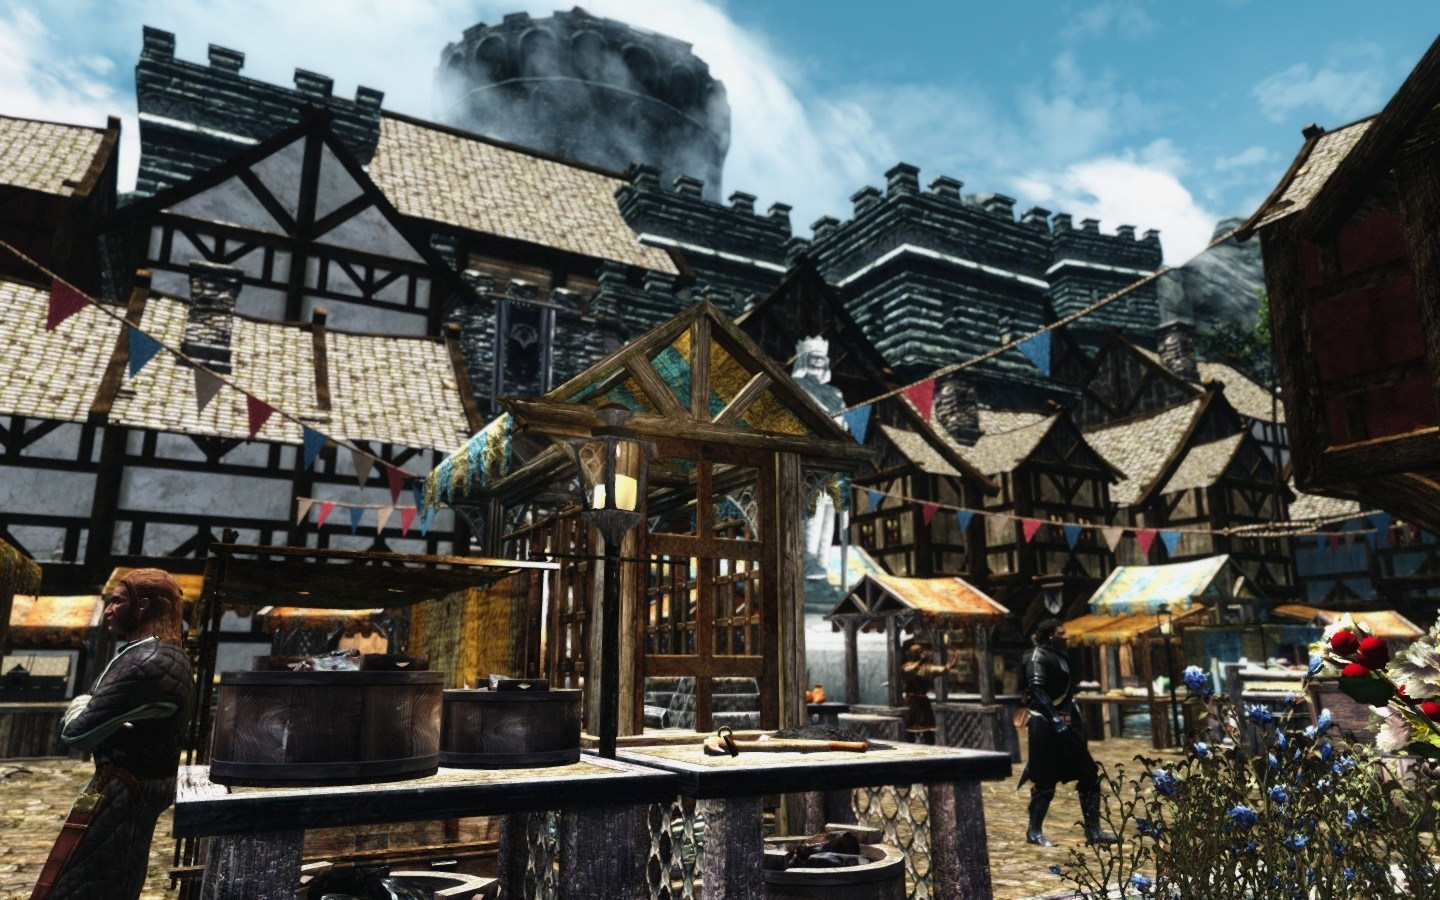
\includegraphics[width=\textwidth]{market.png}
\end{figure}
